\subsection{Selezione di una Rete Bayesiana Esistente}\label{SelezioneRete}

Oltre a poter caricare una rete attraverso l'upload di un file di definizione in formato \textit{JSON} (§\ref{ReteB}) l'utente ha anche la possibilità di selezionare una rete già caricata in precedenza. In questo caso verranno visualizzate nel pannello \textit{G\&B} la rete selezionata con le relative impostazioni di collegamento memorizzate.\\
L'operazione di selezione di una rete bayesiana esistente si articola in due semplici passaggi:
\begin{enumerate}
	\item \textbf{Passaggio 1:} L'utente seleziona, attraverso l'apposito menù a tendina visibile in Figura \ref{SelezioneReteImg} una delle reti bayesiane memorizzate nel server;
	\item \textbf{Passaggio 2:} L'utente conferma il caricamento cliccando il pulsante \textbf{Apri}.
\end{enumerate}

\begin{figure}[H]
	\begin{center}
		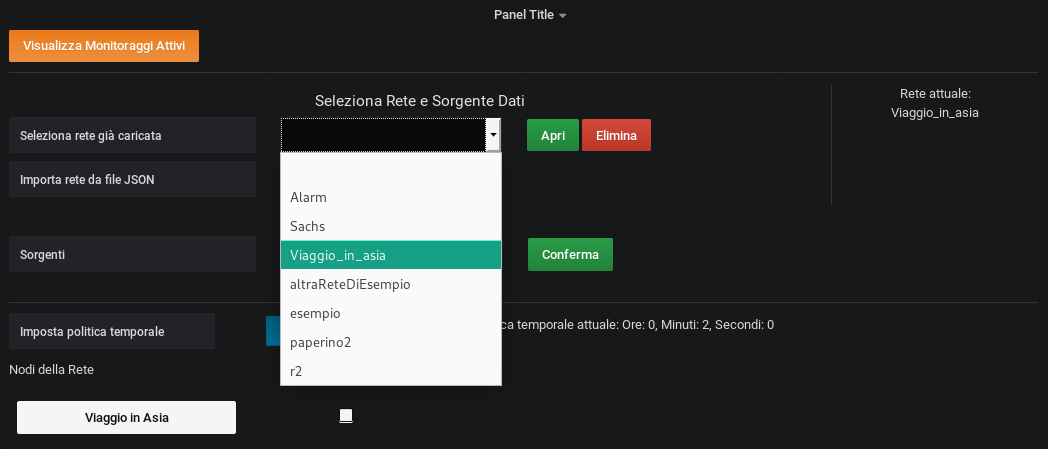
\includegraphics[scale=0.4]{./images/SelezioneRete.png}
		 \caption{Selezione di una Rete Bayesiana già Caricata}	
		 \label{SelezioneReteImg}
	\end{center}
\end{figure}

A seguito del corretto caricamento della rete bayesiana l'utente verrà avvisato del buon esito dell'operazione da un messaggio di notifica (Figura \ref{NotificaSelezioneRete}). Inoltre, nel caso l'utente stesse visualizzando una diversa rete bayesiana prima della selezione questa viene memorizzata nel server insieme alle sue eventuali impostazioni di collegamento.

\begin{figure}[H]
	\begin{center}
		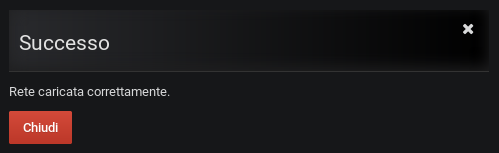
\includegraphics[scale=0.6]{./images/NotificaSelezioneRete.png}
		 \caption{Notifica di Avvenuto Caricamento della Rete Bayesiana}	
		 \label{NotificaSelezioneRete}
	\end{center}
\end{figure}



